\documentclass[10pt,letterpaper]{article} 
\usepackage{tikz}
\usepackage{toolsper}
%\usepackage{graphicx}‎‎
%\usefonttheme{serif}‎
%\usepackage{ptext}‎
%\usepackage{xepersian}
%\settextfont{B Nazanin}
\usepackage{lipsum}
\setlength{\parindent}{0pt}
\newcommand{\pf}{$\blacksquare$}
\newcommand{\EX}{\Bbb E}
\newcommand{\nl}{\newline\newline}
\newcounter{QuestionNumber}
\setcounter{QuestionNumber}{1}

\newcommand{\wid}{40mm}
%\newcommand

\newcommand{\Q}{
\textbf{
سوال \theQuestionNumber)
}
\stepcounter{QuestionNumber}
}
\begin{document}
\Large
\begin{center}
به نام زیبایی

پاسخ تمرینات سری هشتم سیگنال ها و سیستم ها
\hl
\end{center}
\Q

فرکانس زاویه ای نمونه برداری برابر است با:
\qn{
\omega_s={2\pi\over T_s}=20000\pi
}{}
طبق قضیه ی نایکوییست، این مقدار باید حداقل دوبرابر پهنای باند یکطرفه‌ی سیگنال باشد؛ به طور مثال در مورد الف که پهنای باند یکطرفه برابر $5000\pi$ است، دوبرابر این مقدار از فرکانس نمونه برداری کمتر بوده و تداخل رخ نمی دهد؛ در حالی که در مورد ب، پهنای باند یک طرفه برابر $15000\pi$ است که در این مورد، شرط نایکوییست رعایت نشده و تداخل خواهیم داشت.
\nl
پ) چون شرطی روی $\Im$ سیگنال گذاشته نشده است، تداخل می تواند رخ دهد.
\nl
ت) به دلیل تقارن هرمیتیک $X(j\omega)$، می توان گفت تبدیل فوریه‌ی سیگنال آنالوگ در $\omega<-5000\pi$ هم برابر صفر است؛ در نتیجه تداخل مانند قسمت الف رخ نمی دهد.
\nl
ث) به دلیل تقارن هرمیتیک $X(j\omega)$، می توان گفت تبدیل فوریه‌ی سیگنال آنالوگ در $\omega<-15000\pi$ هم برابر صفر است؛ در نتیجه تداخل مانند قسمت ب رخ می دهد.
\nl
ج) چون پهنای باند یک طرفه‌ی $X(j\omega)$ برابر نصف 
$
X(j\omega)*X(j\omega)
$
 است، در حقیقت پهنای باند یک طرفه برابر 
$
15000\pi\over 2
$
 خواهد بود که شرط نایکوییست را ارضا می کند.
\nl
چ) طبق نتیجه گیری 
$$
|X(j\omega)|=0\iff X(j\omega)=0
$$
 و مشابه قسمت الف، تداخل رخ نمی دهد.
\nl
\Q

الف)

اگر تبدیل فوریه‌ی 
$
s_1(t)
$
 و 
$
s_2(t)
$
 را به ترتیب
$
S_1(j\omega)
$
 و 
$
S_2(j\omega)
$
 بنامیم، آنگاه:
$$
Y(j\omega)=S_1(j(\omega-4\pi R))+S_2(j(\omega-6\pi R))
$$

در اینصورت، تبدیل فوریه‌ی آن، مانند شکل 1 است.
\begin{figure}[h!]
\centering
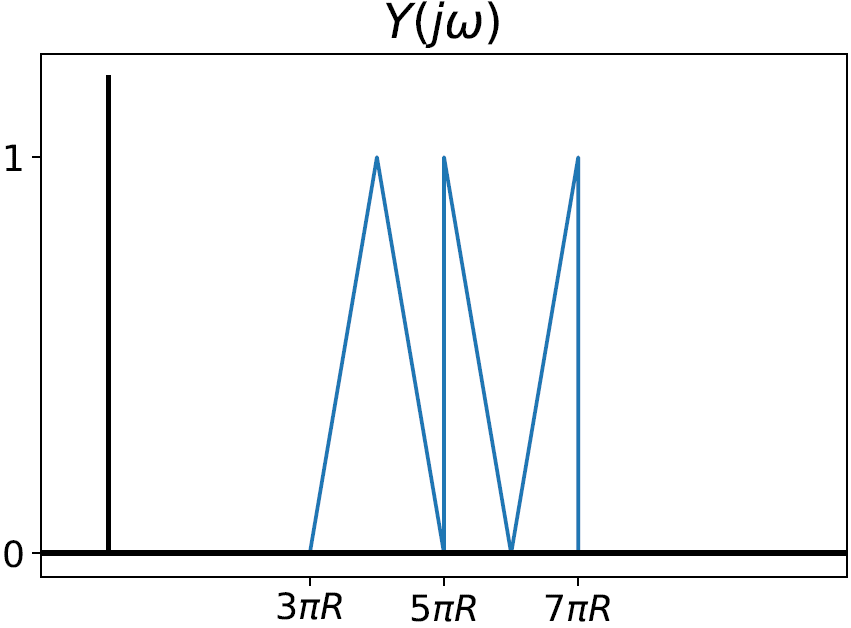
\includegraphics[width=70mm]{PSol8_Q2_1}
\label{fig1}
\caption{تبدیل فوریه ی $y(t)$}
\end{figure}
\nl
ب) از آنجا که پهنای باند طیفی (دو طرفه‌ی) سیگنال $y(t)$، برابر $4\pi R$ است، نرخ نایکوییست نیز باید همین مقدار باشد. اگر نمونه برداری را یا فرکانس $2\pi R$ انجام دهیم، در واقع تبدیل فوریه‌ی $y(t)$ را با دوره تناوب $2\pi R$ در حوزه ی فرکانس شیفت متوالی داده، با خودش جمع کرده و سپس مقیاس فرکانسی را عوض کرده ایم؛ در این صورت:
\begin{figure}[h!]
\centering
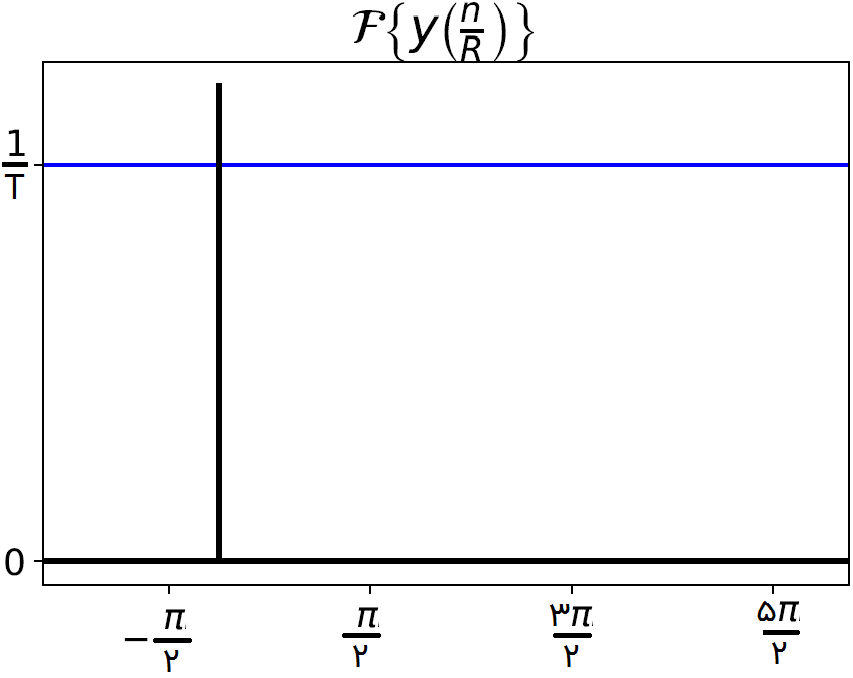
\includegraphics[width=70mm]{PSol8_Q2_2}
%\label{fig1}
%\caption{تبدیل فوریه ی $y(t)$}
\end{figure}
به وضوح، رعایت نکردن شرط نایکوئیست، باعث از بین رفتن اطلاعات طیفی شده است.
\nl
پ) مشابه قسمت قبل:
\begin{figure}[h!]
\centering
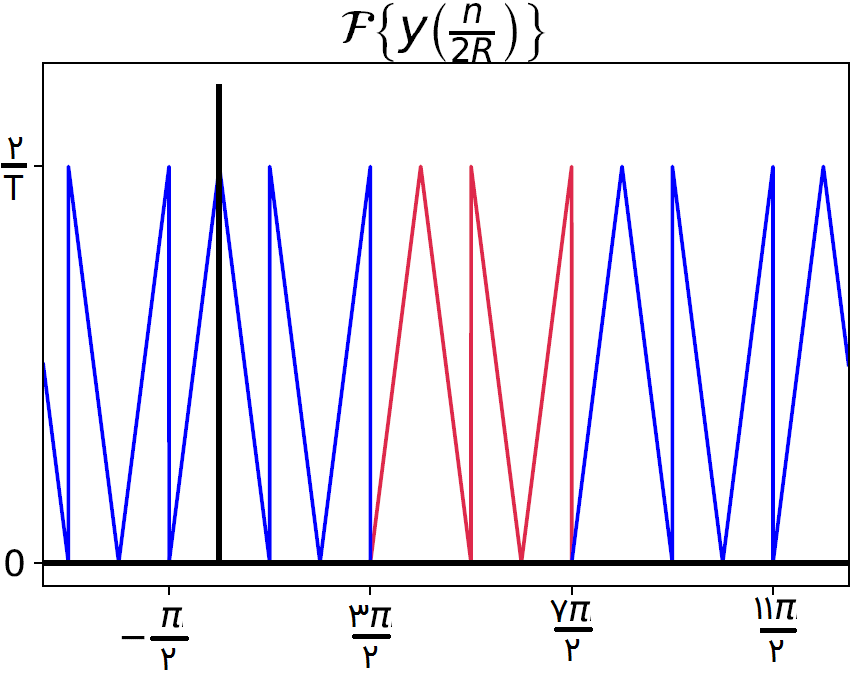
\includegraphics[width=70mm]{PSol8_Q2_3}
%\label{fig1}
%\caption{تبدیل فوریه ی $y(t)$}
\end{figure}
معادل گسسته‌ی تبدیل فوریه‌ی $y(t)$ با قرمز نشان داده شده است.
\nl
ت) تبدیل فوریه‌ی $\hat z[n]$ عبارتست از:
\begin{figure}[h!]
\centering
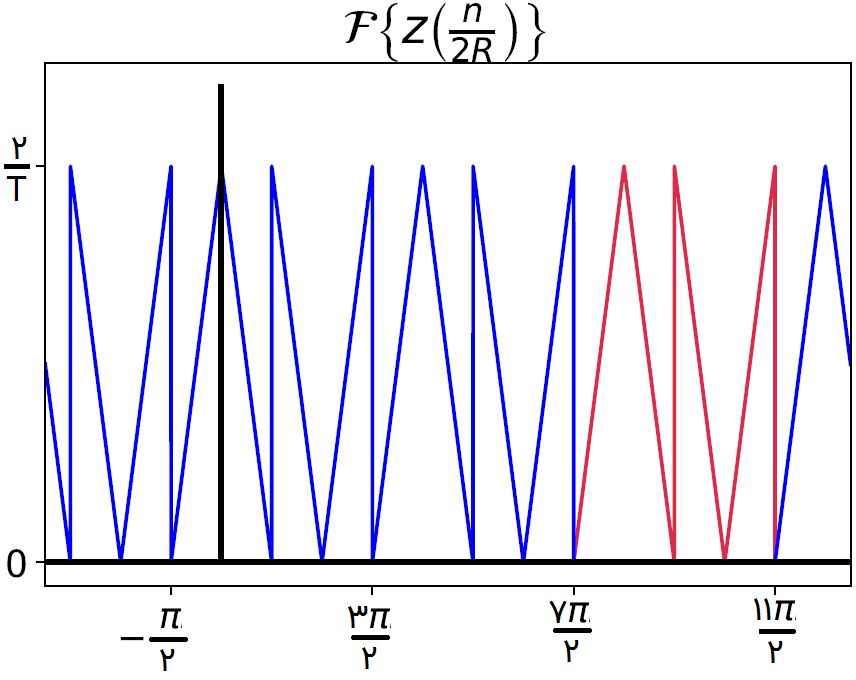
\includegraphics[width=70mm]{PSol8_Q2_4}
%\label{fig1}
%\caption{تبدیل فوریه ی $y(t)$}
\end{figure}
\newpage
که برابر با تبدیل فوریه‌ی $\hat y[n]$ است؛ بنابراین آشکارسازی سیگنال در گیرنده بدون اطلاعات اضافی امکان ناپذیر است. دوباره، معادل گسسته‌ی تبدیل فوریه‌ی $z(t)$ با قرمز نشان داده شده است.
\nl
\Q

از تساوی پارسوال در هر دو حوزه‌ی گسسته و پیوسته بهره می گیریم؛ در این صورت:
\qn{
&E_1={1\over 2\pi}\int_{-\pi}^\pi |X(e^{j\Omega})|^2d\Omega
\\& E_2={1\over 2\pi}\int_{-\infty}^{\infty} |X(j\omega)|^2d\omega
={1\over 2\pi}\int_{-R}^{R} |X(j\omega)|^2d\omega
}{}
از طرفی
$$
X(e^{j\Omega})={1\over T_s}\sum_{k=-\infty}^{\infty}X\left({\Omega-2\pi k\over T_s}\right)
$$
چون تداخل رخ نمی دهد، می توان نوشت:
$$
|X(e^{j\Omega})|^2={1\over T_s^2}\sum_{k=-\infty}^{\infty}\left|X\left({\Omega-2\pi k\over T_s}\right)\right|^2
$$
در نتیجه:
\qn{
E_1&={1\over 2\pi}\int_{-\pi}^\pi |X(e^{j\Omega})|^2d\Omega
\\&={1\over 2\pi}\int_{-\pi}^\pi {1\over T_s^2}\sum_{k=-\infty}^{\infty}\left|X\left({\Omega-2\pi k\over T_s}\right)\right|^2d\Omega
\\&={1\over 2\pi T_s^2}\sum_{k=-\infty}^{\infty}\int_{-\pi}^\pi \left|X\left({\Omega-2\pi k\over T_s}\right)\right|^2d\Omega
}{}
چون فقط یک تناوب از انتگرال بالا در بازه‌ی $[-\pi,\pi]$ می افتد، می توان نوشت:
\qn{
E_1&={1\over 2\pi T_s^2}\sum_{k=-\infty}^{\infty}\int_{-\pi}^\pi \left|X\left({\Omega-2\pi k\over T_s}\right)\right|^2d\Omega
\\&={1\over 2\pi T_s^2}\int_{-\pi}^\pi \left|X\left({\Omega\over T_s}\right)\right|^2d\Omega
\\&={1\over 2\pi T_s}\int_{-{\pi\over T_s}}^{\pi\over T_s} \left|X(\Omega_1)\right|^2d\Omega_1
\\&={1\over 2\pi T_s}\int_{-{\pi\over T_s}}^{\pi\over T_s} \left|X(\Omega_1)\right|^2d\Omega_1
\\&={1\over 2\pi T_s}\int_{-R}^{R} \left|X(\Omega_1)\right|^2d\Omega_1
\\&={E_2\pi T_s}
}{}
تساوی آخر به دلیل برقرار بودن شرط نایکوئیست رخ می دهد.
\nl
\Q

طبق خواص تبدیل فوریه می دانیم:
$$
x[n]=\cos ({\pi\over 4}n+\phi_0)\iff \pi\sum_{k=-\infty}^{\infty} [e^{j\phi_0}\delta(\omega-{\pi\over 4}-2\pi k)+e^{-j\phi_0}\delta(\omega+{\pi\over 4}-2\pi k)]
$$
و
$$
h[n]=\sum_{k=-\infty}^{\infty} \delta[n-4k]\iff
{\pi\over 2}\sum_{k=-\infty}^{\infty} \delta(\omega-{\pi\over 2}k)
$$
بنابراین تبدیل فوریه‌ی 
$
y[n]=x[n]\sum_{k=-\infty}^{\infty} \delta[n-4k]
$
 برابر است با:
\qn{
Y(e^{j\omega})&={1\over 2\pi} \int_{-\pi}^{\pi}X(e^{j\theta})H(e^{j(\omega-\theta)})d\theta
\\&=
{1\over 2\pi} \int_{-\pi}^{\pi}
\pi [e^{j\phi_0}\delta(\theta-{\pi\over 4})+e^{-j\phi_0}\delta(\theta+{\pi\over 4})]
\\&\times 
{\pi\over 2}\sum_{k=-\infty}^{\infty} \delta(\omega-\theta-{\pi\over 2}k)d\theta
\\&=
{\pi\over 4} \int_{-\pi}^{\pi}
[e^{j\phi_0}\delta(\theta-{\pi\over 4})+e^{-j\phi_0}\delta(\theta+{\pi\over 4})]
\\&\times 
\sum_{k=-\infty}^{\infty} \delta(\omega-\theta-{\pi\over 2}k)d\theta
\\&=
{\pi\over 4}\sum_{k=-\infty}^{\infty}
\left[e^{j\phi_0}\delta(\omega-{\pi\over 4}-{\pi\over 2}k)+e^{-j\phi_0}\delta(\omega+{\pi\over 4}-{\pi\over 2}k)\right]
}{}
از طرفی تبدیل فوریه‌ی 
$
{\sin{\pi\over 4}n\over {\pi\over 4}n}
$
 متناوب با $2\pi$ و در بازه‌ی $[-\pi,\pi]$ دارای پالسی در بازه‌ی 
$
[-{\pi\over 4},{\pi\over 4}]
$
 و دامنه ی 4 است. با اعمال این فیلتر به تبدیل فوریه‌ی اخیر، در بازه‌ی $[-\pi,\pi]$  فقط دو ضربه در 
$
\{-{\pi\over 4},{\pi\over 4}\}
$
 خواهیم داشت؛ بنابراین:
\qn{
\mathcal{F}\left\{g[n]*{{\sin{\pi\over 4}n\over {\pi\over 4}n}}\right\}=
{\pi}(e^{j\phi_0}+e^{-j\phi_0})
\sum_{k=-\infty}^{\infty}
\left[
\delta(\omega-{\pi\over 4}-2\pi k)+
\delta(\omega+{\pi\over 4}-2\pi k)
\right]
}{}
بنابراین باید داشته باشیم
$$
e^{j\phi_0}+e^{-j\phi_0}=2e^{j\phi_0}\implies \phi_0=0,\pi
$$
\end{document}